\chapter{Подготовка исходных данных для алгоритма генерации}
\label{cha:code-gen}

Хотя исходными данными для построения модели Крипке служит набор автоматов Мили
(см.~часть~\ref{cha:model-checking}), задавать модель непосредственно в таком виде
неудобно: желательно представлять ее в виде некоторой текстовой нотации.

\section{Выбор используемой нотации}
\label{sec:notation-choice}

В качестве нотации, используемой для задания модели, выбрано подмножество языка Promela,
описанного в разделе~\ref{sec:promela} и используемого в ПО Spin. Это позволяет
использовать модели, созданные для Spin, с минимальными изменениями.

Реализованы следующие возможности языка Promela:
\begin{enumerate}
\item процессы, глобальные и локальные переменные процессов;
\item асинхронные каналы (за один переход к асинхронному каналу может обратиться лишь
  один процесс);
\item операторы \Code{if}, \Code{do}, \Code{atomic}, \Code{print}, \Code{goto},
  \Code{else}, \Code{break}, \Code{skip};
\end{enumerate}

К нереализованным возможностям Promela относятся:
\begin{enumerate}
\item возможность создания новых процессов (все процессы должны быть активны изначально);
\item пользовательские типы данных (структуры и перечисления);
\item синхронные каналы (т.е. каналы нулевого размера, которые представляют собой <<точки
  рандеву>> между двумя процессами);
\item возможность обращаться к явным и скрытым (IP) переменным других процессов.
\end{enumerate}

Грамматика поддерживаемого подмножества языка Promela приведена в
приложении~\ref{cha:promela-grammar}.

\section{Предварительная обработка модели}
\label{sec:idef0-codegen}

В разделе~\ref{sec:seq-algo} приведен алгоритм вычисления множества $Next(s)$ состояний, связанных
с $s$ отношением перехода. В нем вычисляются условия выполнимости текущих инструкций всех
процессов, присутствующих в $s$~--- отсюда мы получаем множество незаблокированных
процессов $P_{ready}(s)$. Далее для каждого процесса $P$ из $P_{ready}(s)$ генерируется
новое состояние, получающееся в результате выполнения его текущей инструкции (номер
которой хранится в $IP_P$). Множество таких состояний и составляет $Next(s)$.

Процесс вычисления $Next(s)$ включает в себя вычисление \Code{Executable} и \Code{Step},
которые которые определяются исходной моделью. Необходимо их представление в достаточно
эффективном для вычисления виде, поскольку разбор и пошаговая интерпретация кода на
Promela может оказаться слишком медленной.

ПО Spin преобразует описание модели в код на языке~C, содержащий реализации функций
\Code{Executable} и \Code{Step} для конкретной модели. В данной работе используется
аналогичный подход~--- исходное описание модели считывается синтаксическим анализатором и
переводится во внутреннее представление в виде графа команд (эквивалентного автомату Мили)
и условий их выполнимости, из которого генерируется код на~С.

Функциональная модель всего процесса предварительной обработки и собственно генерации
состояний на рис.~\ref{fig:stategen-idef0-b0}~и~\ref{fig:stategen-idef0-b1}.

\begin{figure}[ht]
  \centering
  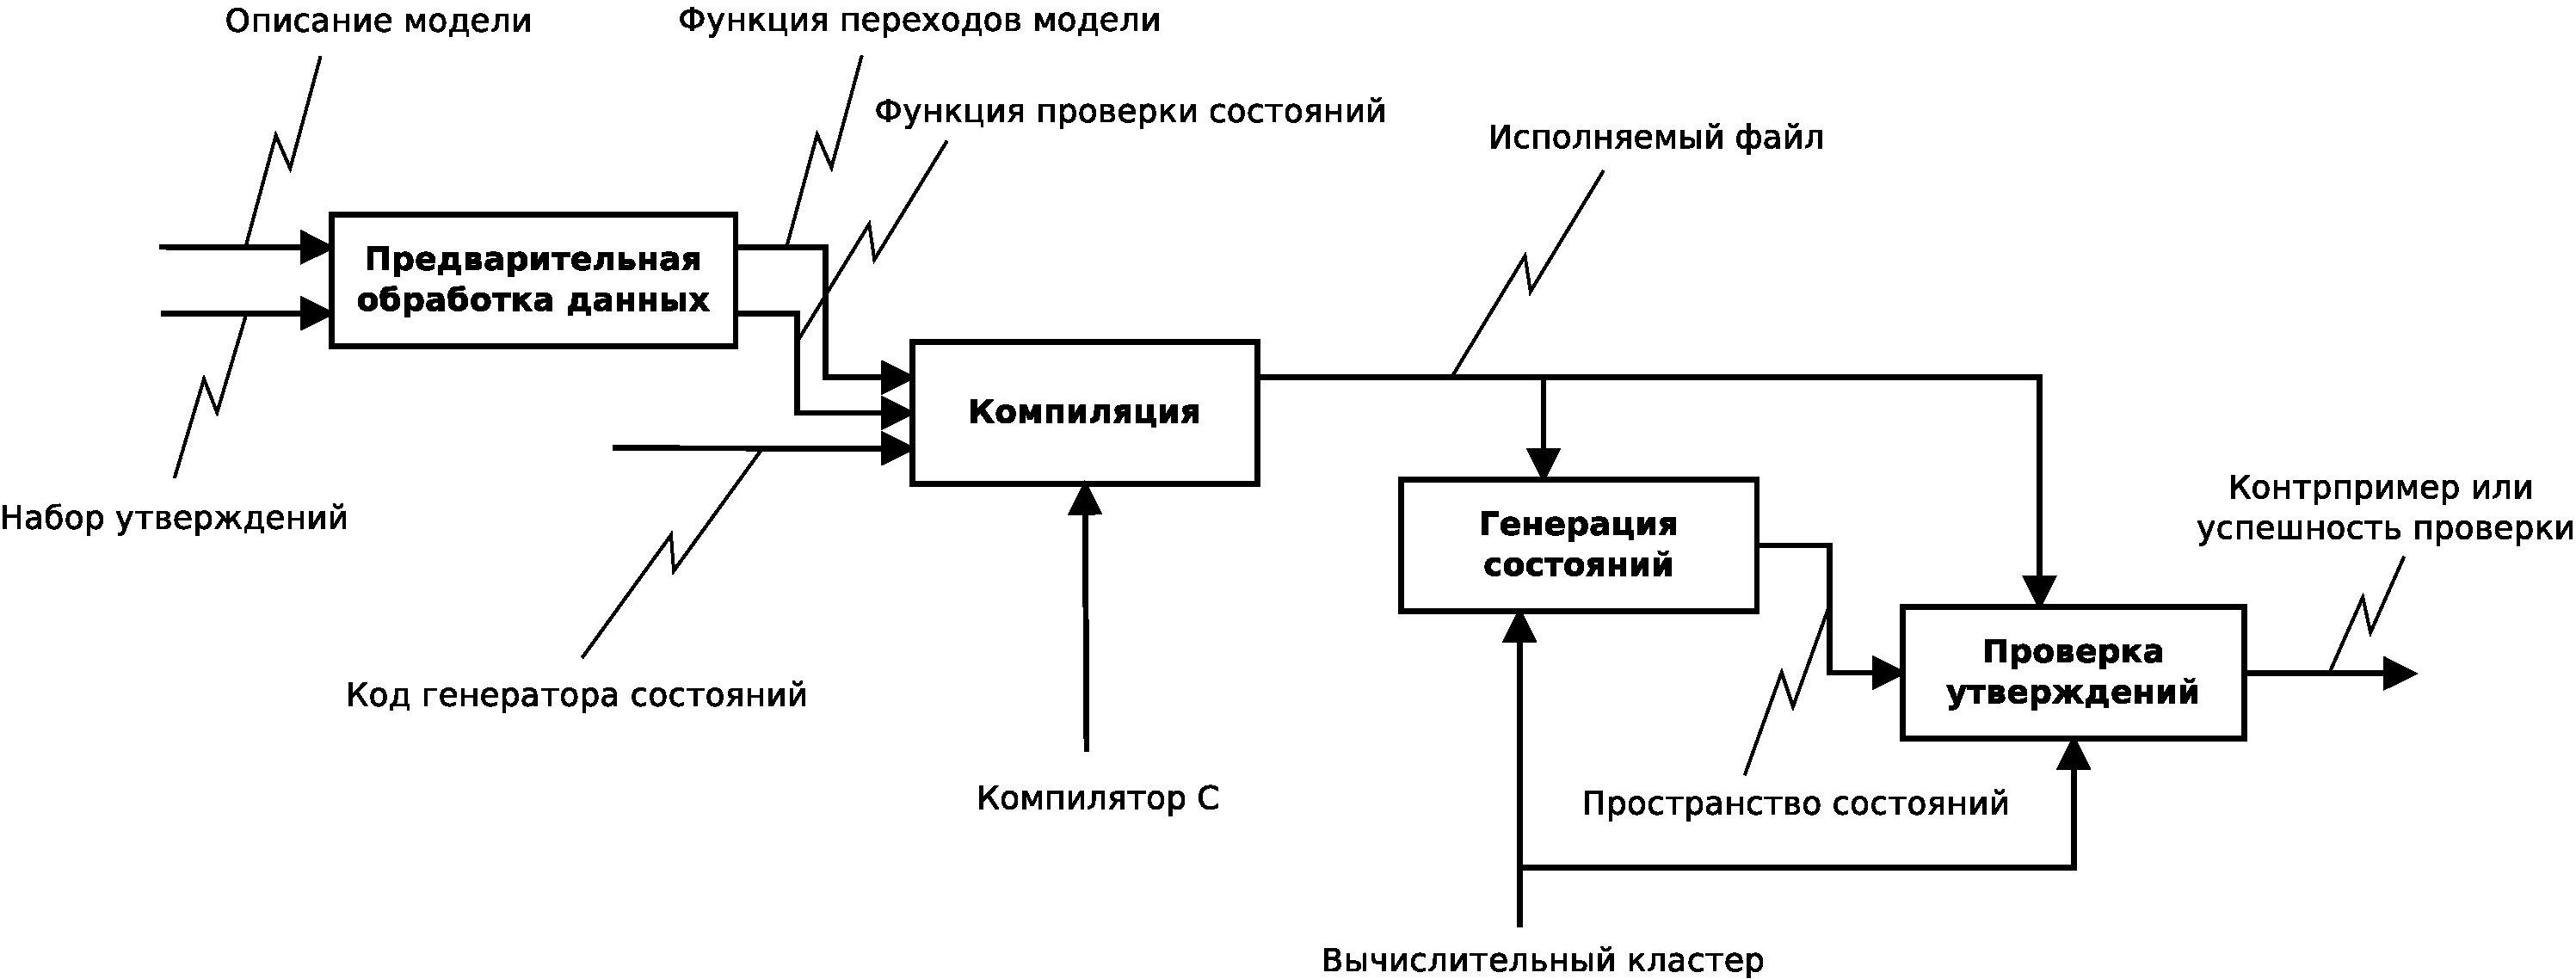
\includegraphics[width=1.1\textwidth]{../graphics/stategen-idef0-b0}
  \caption{Функциональная схема процесса генерации состояний и проверки утверждений}
\label{fig:stategen-idef0-b0}
\end{figure}

\begin{figure}[ht]
  \centering
  \includegraphics[width=1.1\textwidth]{../graphics/stategen-idef0-b1}
  \caption{Функциональная схема процесса предварительной обработки модели}
\label{fig:stategen-idef0-b1}
\end{figure}

Таким образом, генерируются следующие части кода:

\begin{itemize}
\item проверка выполнимости процессов текущего состояния (\Code{Executable});
\item модификация состояния в соответствии с текущей инструкцией выбранного процесса (\Code{Step}); 
\item вспомогательный код (отладочная печать состояния и т.п.).
\end{itemize}

Полученный код компилируется и компонуется вместе с основной программой (обозначенной на
рис.~\ref{fig:stategen-idef0-b0} как <<код генератора состояний>>), осуществляющей выполнение
не зависящих от конкретной модели операций: хэширование и хранение состояний, передача по
сети\etc. Генератор состояний делает вызовы функций сгенерированного кода для вычисления
$Next(s)$, для печати состояния и для инициализации начального состояния $s_0$.

Можно использовать на выбор один из двух генераторов состояний: 

\begin{itemize}
\item последовательный, использованный в разделе~\ref{sec:paremu-test} для имитации параллельного
  выполнения с целью оценки распределения состояний;
\item описанный в главе~\ref{cha:communication} параллельный, использующий MPI.
\end{itemize}

\section{Разбор описания модели и генерация кода}
\label{sec:promela-parser}

Синтаксический анализатор описания модели написан на языке Python. В качестве библиотеки
для синтаксического разбора используется штатный LR(1)-анализатор
\Code{Pyggy}. Преобразование модели во внутренний граф команд (инструкций) и далее в
конечный код осуществляется при помощи СУ-трансляции.

В качестве примера на рис.~\ref{fig:pmlparse-inner} показан граф команд, получающийся для
такого кода:
\begin{lstlisting}[language=Promela]
do
  :: x == 1 -> y = 2
  :: x == 2 -> y = 1
  :: else  -> break
od;
channel1 ! x,y
\end{lstlisting}

Каждая инструкция процесса показана в виде прямоугольника из трех частей: названия,
условия выполнимости \Code{Executable} (в виде выражения на языке~C) и действия перехода
\Code{Step} (аналогично). 

\begin{figure}[ht]
  \centering
  \includegraphics[width=0.9\textwidth]{../graphics/pmlparse-inner}
  \caption{Внутреннее представление модели в виде графа команд}
  \label{fig:pmlparse-inner}
\end{figure}

Большинство инструкций имеет либо тривиальное условие выполнимости \Code{1}, либо
тривиальное действие перехода, обозначаемое как \Code{NOOP}. У инструкций-выражений вроде
\Code{x == 1} тривиальное действие перехода, поскольку их назначение~--- блокировать
процесс, пока не выполняется условие. Инструкции присваивания, как \Code{y = 1}, напротив,
выполнимы всегда. У операторов ветвления \Code{do} и \Code{if} условием выполнимости
является дизъюнкция условий выполнимости всех ветвей (т.е. \Code{do} выполним, если
выполнима хотя бы одна из его ветвей). В тех случаях, когда среди ветвей присутствует
\Code{else}, как в примере, оператор ветвления выполним всегда. Условием выполнимости
самого \Code{else} является отрицание дизъюнкции всех остальных ветвей: он выполним тогда,
когда не выполнима никакая другая ветвь.  

Диаграмма классов транслятора показана на рис.~\ref{fig:pmlparse-classes} в
приложении~\ref{cha:pmlparse-classes}. Среди них выделяется иерархия классов, наследующих
\Code{Expression}~--- описывающих выражения, и иерархия \Code{Statement}~--- описывающих
инструкции различных типов. Классы \Code{Expression} генерируют код на~C для вычисления
выражений языка Promela, а классы \Code{Statement}~--- код вычисления \Code{Executable} и
\Code{Step} различных инструкций.

Каждый тип процесса (\Code{proctype}) описывается экземпляром класса \Code{Process},
содержащего набор инструкций и переменных (\Code{Variable}). Среди переменных выделяются
специальные переменные (\Code{SpecialVariable}), такие как \Code{\_pid}
(см.~раздел~\ref{sec:promela}), и каналы (\Code{Channel}). Каждая переменная имеет свой
тип, описываемый подклассом класса \Code{Type}, задающим операции с этим типом, такие как
объявление в структуре состояния, обращение к переменной данного типа, вывод на
печать\etc.

\section{Представление состояния}
\label{sec:state-represent}

Помимо кода вычисления \Code{Executable} и \Code{Step} генерируются структура \Code{State}
для представления состояния. Она имеет вид, представленный на рис.~\ref{fig:state-repr}.

\begin{figure}[ht]
  \centering
  \includegraphics[width=0.75\textwidth]{../graphics/state-representation}  
  \caption{Представление состояния}
  \label{fig:state-repr}
\end{figure}

Структура \Code{State} включает в себя все глобальные переменные модели, а также поля для
хранения размера (он не определен заранее из-за переменного числа процессов) и атомарности
(<<PID процесса в критической секции>>): при выполнении процессом $P_k$ инструкции
\Code{atomic} в это поле нового состояния $s'$ записывается $k$. В дальнейшем при
вычислении $P_{ready}(s')$ все процессы, кроме указанного в этом поле, будут считаться
невыполнимыми. Когда процесс $P_k$ выполняет последнюю инструкцию в блоке \Code{atomic}, в
поле записывается число $-1$ (оно же и содержится там изначально).

Поля в \Code{State} сортируются по убыванию размера: это связано с тем, что компилятор
может вставлять между ними заполнение (padding) для выравнивания полей размером $B$ на
адрес, кратный $B$, а такое упорядочивание минимизирует объем заполнения.

Непосредственно за глобальными переменными идут структуры с состоянием каждого процесса
$P_i$. Каждому типу процесса (proctype) соответствует своя структура вида
\Code{ProcИмяТипа}, содержащая локальные переменные $IP$ и номер типа процесса. Процессы
хранятся в порядке возрастания их номеров.

Следует отметить, что ввиду ограниченного объема работы не применяется какое-либо сжатие
(см.~раздел~\ref{sec:state-compression}) или упаковка состояний, что приводит к расходу
лишнего объема памяти и делает затруднительной работу на платформах, где требуется
обязательного выраванивание данных, например, MIPS. Более того, передача состояний между
узлами осуществляется также без какого-либо перевода в архитектурно-независимую форму
(вроде пользователького MPI-типа или JSON-объекта). Это означает, что все узлы должны
иметь одинаковую архитектуру (гомогенная вычислительная сеть). Обычно промышленные
кластеры являются гомогенными, поэтому этот недостаток не является критичным.

Ограничения на размер состояния:
\begin{enumerate}
\item максимальное число типов процессов~--- 255; это связано с тем, что поле <<номер тип
  процесса>> 8-битное;
\item максимальное число процессов~--- 254; значение $255$ ($-1$) зарезервировано в поле
  атомарности для обозначения того, что ни один из процессов не находится в блоке
  \Code{atomic};
\item максимальное количество инструкций в процессе~--- 253: поле $IP$ 8-битное, при этом
  каждый процесс имеет две неявных инструкции~--- <<начало>> и <<конец>>;
\item максимальный размер состояния~--- 65536~байт (64~Кбайт), поскольку поле размера
  состояния 16-битное.
\end{enumerate}

\section{Задание проверяемых утверждений}
\label{sec:assertions}

Поддерживается два типа проверяемых утверждений, оба относящиеся к классу условий
<<надежности>>.

\paragraph{Проверка значений переменных}

Проверка значений переменных в определенных переходах осуществляется при помощи встроенной
в язык Promela функции \Code{assert} (см.~раздел~\ref{sec:spin}). Как и в ПО Spin,
\Code{assert} является самостоятельной инструкцией, приводящей к генерации отдельного
состояния. Инструкция \Code{assert} всегда выполнима, и при ее выполнении вычисляется
значение указанного выражения. Если оно равно $0$, результат свойств проверки модели
считается отрицательным, текущее состояние предоставляется в качестве контрпримера $s_e$,
и дальнейшая генерация состояний прекращается.

\paragraph{Недопустимые финальные состояния}

Опционально можно включить проверку финальных состояний: она заключается в том, что $IP$
всех процессов в финальных состояниях должны указывать на последнюю инструкцию
(<<конец>>). Проверку финальных состояний можно использовать для поиска мертвых блокировок
в параллельных алгоритмах и протоколах, в частности, в разделе~\ref{sec:kripke-verification}
приводится пример, как с ее помощью обнаруживается мертвая блокировка в задаче о
философах.

\section{Тестирование транслятора модели}
\label{sec:pmlparse-testing}

Проводилось модульное и функциональное тестирование реализованного транслятора языка
Promela.

\paragraph{Модульное тестирование}

Модульное тестирование проводилось по критерию C1 (покрытие всех ветвей). Тесты
составлялись вручную с применением библиотеки \Code{unittest}, пример использования для
тестирования классов-инструкций (\Code{Statement}) которой показан далее.

\lstinputlisting[language=Python,style=realcode]{../data/inc/t-statement.py}

\paragraph{Функциональное тестирование}

Поскольку единственным результатом работы транслятора является код на языке~С, реализующий
функцию переходов модели \Code{Next}, в ходе автоматического системного тестирования
проводилось сравнение получаемого кода для заданных тестовых примеров входных моделей.

Выделяются следующие классы эквивалентности.
\begin{enumerate}
\item Входная модель содержит синтаксические ошибки.
\item Входная модель не содержит переменных.
\item Входная модель содержит лишь глобальные переменные.
\item Входная модель содержит лишь локальные переменные процессов.
\item Входная модель содержит как глобальные, так локальные переменные.
\item Входная модель состоит из процессов одного типа.
\item Входная модель состоит из процессов различного типа.
\item Входная модель содержит каналы.
\item Входная модель содержит атомарные блоки.
\end{enumerate}

%%% Local Variables: 
%%% mode: latex
%%% TeX-master: "thesis"
%%% End: 
